%% Support sites:
%% http://www.michaelshell.org/tex/ieeetran/
%% http://www.ctan.org/tex-archive/macros/latex/contrib/IEEEtran/
%% and
%% http://www.ieee.org/
%****************************************************************

\documentclass[pdf,bookmarks,colorlinks=true]{IEEEtran}
\usepackage{times}
\usepackage{amsmath}
\usepackage{hyperref}
\usepackage{url}
\usepackage{psfrag}    %Shouldn't use this if you plan on using pdflatex!
\usepackage{graphicx}
\usepackage{wrapfig}   %for wrapping text around figures and tables
\usepackage{graphicx}

\makeatletter
\def\endthebibliography{%
	\def\@noitemerr{\@latex@warning{Empty `thebibliography' environment}}%
	\endlist
}
\makeatother

\begin{document}
%
% paper title
% can use linebreaks \\ within to get better formatting as desired
% Do not put math or special symbols in the title.
\title{Review of Cybersecurity in the Radiology Department}


\author{Leonardo Arthur Pangemanan\\
	Southern Adventist University\\
	lpangemanan@southern.edu
}



% The paper headers
\markboth{CPTE-542-A Survey Paper, October 2019}%
{Shell \MakeLowercase{\textit{et al.}}: CPTE-542-A Survey Paper, October 2019}

\maketitle

% As a general rule, do not put math, special symbols or citations
% in the abstract or keywords.
\begin{abstract}
	Cybersecurity is an increasing concern for many healthcare organizations, information technology and medical cybersecurity professionals. As more computerized medical devices become connected to the network within and outside the facility increases, the risk of cyber attacks also increases. Moreover, the radiology departments have most of their devices connected to the network. Most radiologists are unaware of the vulnerability of their devices. This paper will review the cyber threat of modern medical devices within the radiology department to build more awareness to these vulnerabilities.
\end{abstract}

\section{Introduction}
\IEEEPARstart{T}{he} healthcare industry has change ever since the first computer were introduced. The healthcare technologies have the potential to extend, save and enhance the live of patients. Furthermore, hospitals have witnessed a proliferation of networked medical equipment in the past decade. There is an emergent trend of connecting medical equipment to the hospital network for easy accessibility and manageability. As healthcare devices continue to evolve, so does the inter-connectivity. For example, it provides efficiency, error reduction, automation, and remote monitoring. Interconnected technology allows health professionals to monitor and adjust devices without the need for hospital visit or invasive procedure \cite{coventry2018cybersecurity}. With integration comes complexity and challenges in management and this protection \cite{williams2015cybersecurity}. However, interconnected technology introduces new cyber-security vulnerabilities in the same way other networked computing systems are vulnerable. Recently, securing medical devices against cyber attacks or malware outbreaks and safeguarding protected health information (PHI) stored on devices or exchanged between a device and the provider's network is a growing challenge for clinical engineers and hospital information technology (IT) professional \cite{wirth2011cybercrimes}. The number of high-profile public demonstrations of successful attacks on devices and medical networks have increased. This fact raises the concern that inter-connectivity will directly affect clinical care and patient safety. \par
% New Paragraph
Over the past few years, the question of inadequate clinical security has been gaining attention from both industry leaders and clinical practitioners. The integration of medical devices, networking, software, and operating systems means that the relative isolation and safety of medical devices are challenged \cite{williams2015cybersecurity}. These vulnerability is also due to many manufacturers focus their efforts on innovation and functionality, with little emphasis on the network security of this devices \cite{moses2015lack}. \par
Designing a secure medical device is fundamentally different from  any other devices that only focus on safety and efficacy. Safety design decisions are based on the assumption that hazardous condition or failure occur accidentally. However, the assumption that hazardous condition or failure occurs accidentally no longer holds true as malicious attackers try to trigger hazards in devices through intentional repeated attempts \cite{Ray}. Thus manufacturer tends to not implement the necessary security check against these malicious attacks. This fact become more important as the radiology departments usually have the highest density of networked medical equipment in a hospital \cite{moses2015lack}. 

The rest of this paper first discusses the background of cyber security in
\ref{sec:Background}, and then describes my main topic in
\ref{sec:Radiology}. Lastly, \ref{sec:Conclusion} presents the
conclusions and describes future work.

\begin{table*}[tbh]
	\caption{Common cyber threats in healthcare \cite{martin2017cybersecurity}.}
	\centering
	\begin{tabular}{l l}
		\hline\hline
	Data theft for financial gain & Stealing personal data for the purposes of monetary gain. \\
	Data theft for impact & Theft and public release of sensitive medical information. \\
	Ransomware & Using malware to block users from their data or systems or to delete data unless a fee is paid. \\
	Data corruption & Deliberate corruptions of data, such as altering test results, for political or personal gain. \\
	Denial of service attacks & Disruption of a network or system by flooding it with superfluous requests motivated by blackmail, revenge, or activism. \\
	Business email compromise & Creating fake personal communications for financial gain.\\ 
	The unwitting insider & Substantial disruption to systems or the loss of data owing to the unintentional actions of staff using outdated and at-risk systems. \\
	\hline
	\end{tabular}
	\label{tab:common}
\end{table*}

\section{Background}
\label{sec:Background}
With the numerous data breaches in healthcare over the last several year, it seems to be unreasonable for patients having any expectation of privacy and security in their health information. In 2012, 780,000 patients records were stolen from the State of Utah Department of Health, Department of Technology server, by an Eastern European hacker. Another at Saint Joseph's Health System in California, approximately 31,800 patients' record was made potentially available through basic Internet search engines for about a year because security settings on the system were set incorrectly \cite{murphy2015cybersecurity}. Increasingly, healthcare is a prime target for cyber attack with a recent SANS Institute report reporting that 94\% of healthcare organization have been the victim of a cyber attack \cite{williams2015cybersecurity}. Table \ref{tab:common} shows the most common cyber attacks healthcare organizations is vulnerable to. In May 2017, a ransomware called WannaCry infect more than 200,00 computers in 150 countries. One of the victim was the National Health Services (NHS) in the United Kingdom. Nearly 19,000 appointments had to be canceled, costing them and estimate \pounds20 million. The NHS spent an additional \pounds72 million to recover from the disaster and upgrade its systems \cite{ferrara2019cybersecurity}. The vulnerability of healthcare to cyber attack reflects a combination of factors, notably limited resources, fragmented governance, and cultural behavior. \par
In May 2017, The Ponemon Institute shared a survey that showed only 15\% of healthcare delivery organization (HDOs) and 17\% of medical device manufacturers (MDMs) were taking significant steps to prevent cyber attacks \cite{busdicker2017role}. Figure \ref{fig:total-number-of-malware-per-year} shows the total number of malware that is on the internet. With this many malware, there should be a protection against them. However, most healthcare organization exist to provide cybersecurity within their devices. The industry more focuses on providing healthcare to the patients in need. Their revenue or reimbursement for healthcare is not tied to any cybersecurity effort. More importantly, there is a traditional believes that no one would be motivated to attack healthcare systems and protective measure were not necessary. As mentioned before, many of these healthcare organization ignore the potential danger of cyber attack and solely focus on giving patient care \cite{coventry2018cybersecurity}. Moreover, the healthcare industry is one of the most targeted sectors globally; 81\% of 223 organizations surveyed, and $>$110 million patients in the United States had their data compromised in 2015 \cite{martin2017cybersecurity}. Currently, there are many motivations for hackers to attack healthcare organizations and professional needs to increase the priority to enhance their cybersecurity.

\subsection{Cybersecurity Terminology}
Cybersecurity terms are unfamiliar to many people and can leads to misunderstanding by those who do not work in the cybersecurity or information technology professions. Here are the most common terms associated with cybersecurity \cite{ferrara2019cybersecurity}:
\begin{itemize}
	\item {\bf Distributed Denial of Service (DDoS)}: a cyber attack where the hacker use multiple device to send a request to a website or a network. If the number of requests is large enough, the website or network cannot handle the traffic and stop responding, therefore preventing legitimate users from accessing the network.
	\item {\bf Malware}: Typically a software designed to interfere with the computer's normal function. This interference can take the form of destruction of data, inability to run the computer or certain programs, stealing personal information, or causing physical damages to the device. The different types of malware include:
	\begin{itemize}
		\item 
		
	\end{itemize}
\end{itemize}


\begin{figure*}[tp]
	\centering
	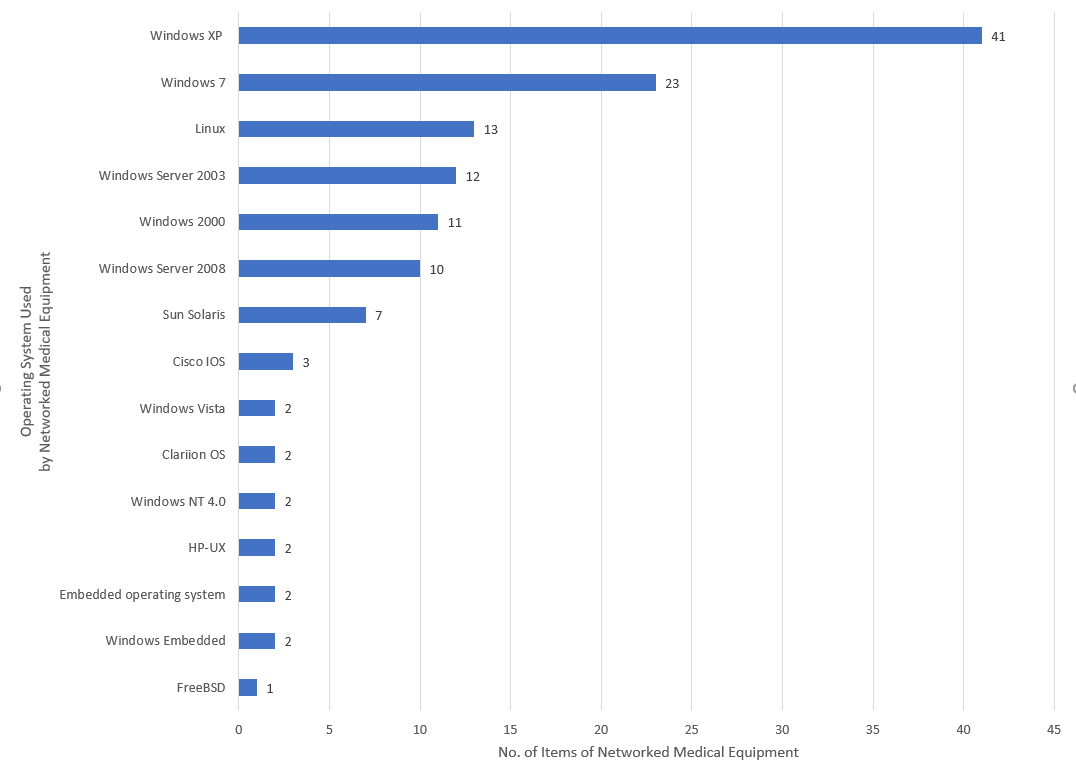
\includegraphics[width=0.7\linewidth]{OSonRadiology}
	\caption{The distribution of Operating System running on networked medical equipment in the radiology department \cite{moses2015lack}.}
	\label{fig:osonradiology}
\end{figure*}

 
\subsection{Implantable Medical Devices}
\emph{Implantable Medical Devices} (IMDs) apply continuous monitoring and automatic therapies to the treatment of chronic medical disorders \cite{Rostami:2013:HAI:2541806.2516658}. For example, a typical IMDs monitor and treat physiological conditions within the body and improve patients' quality of life and help sustain their lives.  These devices includes pacemakers, implantable cardiac defibrillators (ICDs), drug delivery systems, and neurostimulator. With these devices, health professional can treat abnormal physiological conditions within the body, such as cardiac arrhythmia, diabetes, and Parkinson's disease. IMDs' pervasiveness continues with upward of 25 million United States citizens currently reliant on them for life-critical functions \cite{halperin2008security}. In the United States, over 100,00 patients a year receive implantable cardioverter defibrillators (ICDs), which detect dangerous heart rhythms and administer electric shocks to restore normal activity \cite{Rostami:2013:HAI:2541806.2516658}. Some current-generation devices now have the ability to communicate wirelessly with external equipment from distances up to five meters away \cite{denning2010patients}. In fact, the latest IMDs is able to support remote monitoring over long-range, high-bandwidth wireless links, and emerging devices will communicate with other inter-operating IMDs. \par
Despite these advances in IMD technologies, they still can occasionally malfunction. Additionally, they are still behind in security and privacy. Many information technology professionals are still lacking in the understanding of how device security and privacy interact with and affect medical safety and treatment efficacy. Cybersecurity protection of these devices are not just a technical issue according to \cite{williams2015cybersecurity}. The foundational study of these devices demonstrated the vulnerability is detrimental to their safe operation, and the availability, confidentiality, and integrity ot the associated data. IMDs poses the challenge of having a balance of security and accessibility for medical professionals.	

\begin{figure*}
	\centering
	\includegraphics[width=0.7\linewidth]{"Total Number Of Malware per Year"}
	\caption{A graph of total number of Malware per year, based on data from AV-TEST \cite{AVtest}.}
	\label{fig:total-number-of-malware-per-year}
\end{figure*}


\section{Cybersecurity in Radiology Department}
\label{sec:Radiology}
Healthcare today increasingly depends on computers, networking, and information system. Due to the need of digital healthcare, most diagnostic imaging systems are connected to the Internet/LAN (Local Area Network) \cite{ma2019medical}. Furthermore, this connectivity enables computer enhanced medical imaging capabilities, that allows for early discovery of diseases, research new diseases, and better treatment of medical condition.  The radiology department specifically, have seen a more proliferation of networked equipment in the past decades. They also have the highest density of networked medical equipment. Many manufacturers focus solely on innovation and functionality but little effort was put on the network security of this equipment. Also, digital storage and transmission of images across the hospital network using PACS have become a well-established norm in most large radiology departments \cite{moses2015lack}. 

\subsection{Types of Cyber Threats}

\subsection{Security Challenges}
The medical industry face many challenges 

\section{Conclusion And Future Work}
\label{sec:Conclusion}

Many researcher try to make a secure systems for the healthcare industry. For example, \cite{Almohri:2017:TMM:3204094.3204113} made a threat modeling and mitigation of medical cyber physical systems. 


%--- bibliography ---
\bibliographystyle{IEEEtran}

\bibliography{reference}
% that's all folks
\end{document}


